In this body of work we have taken some important steps forward. We have provided a state of the art way to trace student knowledge, we have found a strong natural pattern in how students navigate problem spaces and we have broken ground on the problem of how to understand the sparse solution space of richly structured assignments. Despite these achievements, there is a large amount of work left to do. In the process of working on a range of challenges in this domain I have developed a sense of what works and what lines of thought I believe will be part of the future of autonomous understanding of students. Here are some of the most fruitful ways forward, in my opinion. 


\section{Deep Tutor}

The Deep Knowledge Tracing project is a stepping stone that opens up several new veins of research that have the potential to revolutionize our ability to autonomously provide feedback. The two most obvious ways forward are (1) unlike the bayesian networks that were the previous state of the art, recurent neural networks take vectors as input. Can can leverage this to allow knowledge tracing to evolve beyond the domain of correct/incorrect problems? (2) we now can model what students know. Can we optimize our ability to make feedback decisions?

(1) My focus so far has been on how to understand students, and I waited on the question of how to deliver feedback. The second half of the equation, the actual delivery of hints is a hard problem. However the machine learning community has made substantial progress in solving similar domain of tasks. The Deep Mind group published the results of a project called Deep Q Learning \cite{mnih2015human} that is particularly inspiring. The core idea of the article is simple. Build and train a neural network function that can takes raw inputs and outputs a prediction of the ``Q-function" -- a utility value for the given world-state and all actions taken at that state. The loss value that is backpropagated through the neural network is set by its ability to satisfy the Bellman Equations for Markov Decision Processes. Using their neural network they showed incredible proficiency at making decisions in the context of Atari games where the only inputs it was given were raw pixel data. It often performs substantially better than human experts at the games. This project was inspiring because it is feasible to cast the tutoring task, chosing what hint to give to a student and chosing what problem a student should solve next, as a game. This game doesn't have pixels, instead we observe how students solve problems. And instead of points, the goal of the game is to maximize student learning.

Given the success of Deep Knowledge Tracing at being able to understand what students know, and represent that knowledge in euclidean space, it seems very believable that it could be used as a basis for a Deep Tutor. The central difference between an Atari game and modelling a student is that an Atari game is genuinely markovian. The Deep Mind team made Q-predictions only using pixels from the previous 5 frames. Those frames contained everything the model needed to know. In contrast, we would like predictions in the context of students to take into account long term memory of the students actions. The Deep Knowledge Tracing model that we generated can turn the long term memory of a students actions into a single vector. Thus it could be extended so that at each point we use the vector representing the memory of a students actions to both predict if a student will answer a question correctly \emph{and} also predict the Q-Value for all possible tutor actions. In the setting of autonomous tutoring, an action could be anything from providing a hint, to selecting a next question, to pointing the student to a relevant resource. The resulting model as applied to correct/incorrect problems (such as the ones in Khan Academy) is shown in figure \ref{fig:deepTutor_basic}. If we can use a neural network to help make tutoring decisions, we could have autonomous tutors which help students in subtle and rich ways, taking into account a long view of their learning, both in terms of understanding the learner's past, and in predicting their future.


 \begin{figure*}[ht]
 \centering
 \subfigure[]
 {
 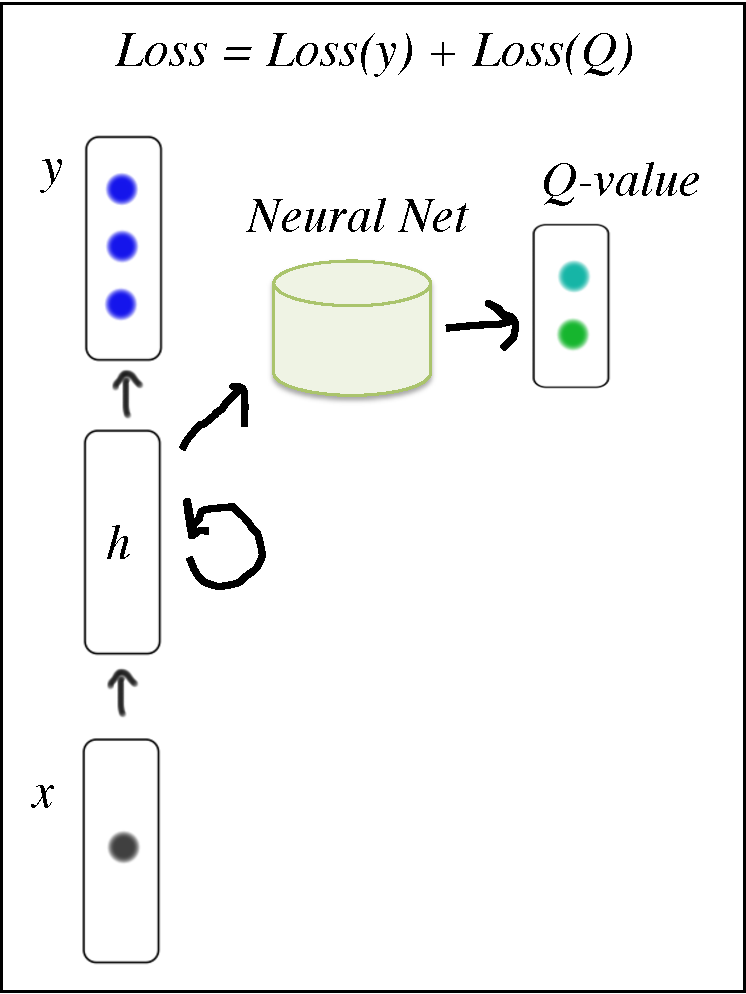
\includegraphics[width=0.35\textwidth]{img/deepTutor_basic}
 \label{fig:deepTutor_basic}
 }
 \subfigure[]
 {
 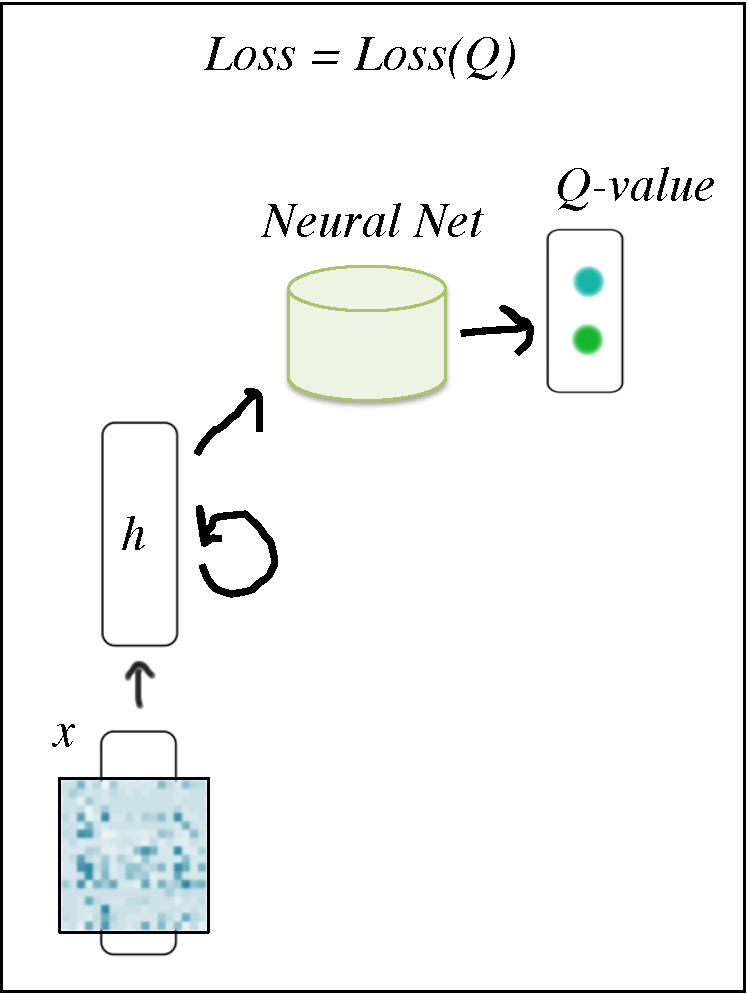
\includegraphics[width=0.35\textwidth]{img/deepTutor_vector}
 \label{fig:deepTutor_vector}
 }
 
 \caption[Deep tutor models]{Deep Tutor models for inputs that are (a) encoded as correct/incorrect (b) encoded as vectors.}

 \end{figure*}

A small group of colleagues and I have taken the first steps to explore this idea. We set up a synthetic tutoring game where randomly generated students answer synthetic questions and a computer choses what question a student solves so as to maximize their knowledge after a fixed amount of time. This ``game" is based, to the best of our ability, on learning science theories. The autonomous tutor (player) is not given under the hood information and has to learn to make its decisions off of student interactions. Since the game is synthetic it is well understood. We know the theoretical optimal strategy and can understand how close the player is to discovering said strategy. Our vanilla implementation of The Deep Knowledge Tracing model combined with Q-function prediction substantially outperforms baseline methods. We hope to learn what modifications of the model allow it to achieve optimal performance. Given a strong showing on a synthetic dataset, the next step -- just as in the DKT paper -- is to show that it also works on real student data.

(2) One of the promises of Deep Knowledge Tracing is that it will allow the practice of knowledge tracing to extend beyond correct or incorrect answers. While bayesian models were best suited for educational signals that were discrete, in DKT models, the input of a students interaction is a vector. We are excitingly close to being able to model knowledge for anything that can be embedded into a reasonable euclidean space. One example of the difference that will make is highlighted by our project on embedding programs into euclidean space. DKT, it seems, should be able to build its model of what students know off of these complex inputs. However, there is one unsolved problem that needs to be tackled first. The prediction output of neural networks is also a vector. And as such we could interpret the vector as we like and build a loss function based on a difference between the vector output and the true value that is being predicted. In the case of programs, the output would be a vector which we would interpret as the program the model predicts the student will write next. The issue is that by only predicting one point in a high dimensional space, there is no way to articulate that a soft distribution of programs is to be expected. My untested hypothesis is that is will limit the effectiveness of such a strategy. The problem, in short, is that vector inputs are easy to handle. Loss functions over vector outputs are more complicated. A very interesting and open question, both for the field of education and for the field of machine learning, is how can we compute a soft loss prediction of an entity for which we know vectorizations? 
However, a potentially important observation is that maybe we don't need the loss to be based on a prediction of what vector output the student will produce next. Possibly, we could rely on another form of loss. The Q-function prediction might provide enough loss to learn structure. As such a model such as the one in figure \ref{fig:deepTutor_vector} might jointly solve both the problem of how to handle complex inputs \emph{and} the problem of how to make decisions based on understanding.

If we could solve either, or both, of these problems we would substantively change the nature of autonomous tutoring. Both in the domain of education actions to which it could apply and in the ability to turn 

\section{Better Program Encodings}

Understanding the sparse space of student programs remains an open problem, and one that is foundational to further advances in understanding students as they program. In this thesis we explored two seperate methods to find patterns amongst a set of student programs. In simpler domains, such as correct/incorrect problems, machine learning tools are especially useful at understanding temporal student patterns. To me this suggests that while the problem of learning how to embed programs into euclidean space is difficult, it is the prefereable strategy to pursue. I still believe that embedding Hoare tripples was a good one, but there is always a better way. And for this particular problem: how to predict post-condition given pre-condition and code, there are many other models that are worth trying. Several of the leading experts in neural network (for example Jürgen Schmidhuber) are actively trying to teach programs how to ``compute" programs. If substantial progress is made it would be directly useful for education reserach.

It is possible that in order to imporve our ability to project programs into vector space, we may need to come up with a richer objective function. In many education settings there are copious amounts of human annotations on student programs, both in the form of rubrics and comments. Using these sources to understand program similarity might be a crucially important step. It would be particularly interesting to see to what extent teacher assessment translates to student progress and the Poisson Path from the student's final submission to the solution.

Another angle worth considering is to use sequences of outputs of programs (executed on standard inputs) as the raw data that we use to encode programs. You could think of a program's execution on unit tests as a set of movies. Substantial progress is being made in understanding video, maybe this will be able to translate into understanding programs. An obvious difference is that often programs have human interaction. However this is a challenge that has been thuroughly adressed by the program testing community.


\section{Pivot to offline}
In this thesis we used online learning as a case student to explore our ability to understand learners. While this was a practical necessity it paints a bleak picture of the future of education. If we want our children (or our grandchildren) to have the best education possible, will they have to sit infront of a screen for as long as possible? My hypothesis is that, while screens may be a necesity for the short term, in the long term the answer will be no. Even for computer science, it will be useful to have time interacting with different mediums. Maybe children will sit at a desk with something akin to an Amazon Echo strapped to a camera (possibly with cute eyes so that it looks less threatening) that watches us as we work through problems, understands our learning, and gives us feedback. If we want something better than the lousy vision I just proposed, it will require research into new mediums of learning that enable deep understanding and are more engaging and healthy for students.

A potential way to enter into this field of research is via understanding exam grading. At Stanford, as well as at other institutions, when students take computer science or math exams they often hand write their answers. This makes administering exams especially easy and means that students with worse computers are not at a dissadvantage. These hand written programs are then laboriously graded by a team of teaching staff. If the exams are first digitalized then not only could grading be faster, but they could be more accurately assessed. And, importantly, their learning could be tracked in a meaningful way across time. This would be a powerful demonstration of how maching learning applied to understanding human learning could work for offline education.

\section{Final Note}
The future of technology advances for understanding students is rich. I am truly excited to see what happens. If you find yourself reading this and you are interested in talking, please feel free to reach out. I imagine regardless of where life takes me I will always be interested to see where this field of research goes. Thank you for taking the time to read my thesis.